\chapter{Breadth First Search - BFS}
Visita in ampiezza di un grafo non orientato
\section{Introduzione Concetti}
\subsection*{Distanza tra due vertici}
$G=(V,E) \rt$ grafo non orientato con insieme V dei vertici e insieme E degli archi.\\
\textbf{Distanza} di u da v \ra minimo numero di archi da percorrere per andare da v a u.
\paragraph*{Esempio} Distanza di 3 da 4 = 2
\begin{center}
    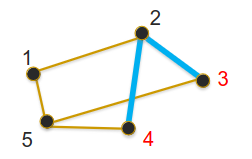
\includegraphics[width=80mm, scale=0.5]{bfs-esempio-pesi.png}
\end{center}
In poche parole è come se ogni arco avesse peso 1.
\subsection*{BFS(G,s) - Visita in ampiezza}
Significa effettuare la visita di un grafo \textbf{non} orientato G, a partire da un vertice
sorgente s:
\begin{itemize}
    \item All'inizio viene visitata la sorgente s
    \item Vengono poi visitati uno dopo l'altro tutti gli adiacenti di S
    \item In seguito, per ogni adiacente v di s, vengono visitati uno dopo l'altro
    gli adiacenti di v non ancora visitati
    \item Si prosegue a visitare gli adiacenti degli adiacenti e via di seguito
\end{itemize}
Tradotto in un esempio pratico:
\begin{itemize}
    \item Viene visitato s
    \item Vengono visitati tutti i vertici a distanza 1 da s
    \item Vengono visitati tutti i vertici a distanza 2 da s
    \item Vengono visitati tutti i vertici a distanza 3 da s
    \item etc.
\end{itemize}
\subsection{Caratteristiche di BFS}
\begin{itemize}
    \item Visita tutti e i soli vertici raggiungibili da s (vedremo che per DFS non sarà così)
    \item Ogni vertice del grafo viene visitato al più una volta
    \item Permette di trovare la distanza (in archi) da s di tutti i vertici
    raggiungibili dalla sorgente
\end{itemize}
\section{Colore Vertici}
I vertici hanno associato un colore:
\begin{itemize}
    \item vertice \underline{bianco} \ra vertice non visitato
    \item vertice \underline{grigio} \ra vertice visitato (adiacenti non
    completamente visitati)
    \item vertice \underline{nero} \ra vertice visitato (adiacenti completamente visitati)
\end{itemize}
\section{Esempio Esecuzione BFS}
BFS(G, A), in questo modo identifico che la sorgente è A, quindi inizio da A.
\begin{center}
    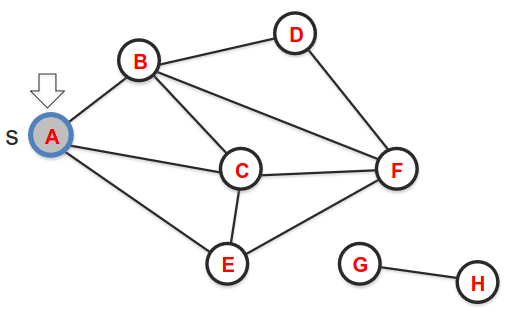
\includegraphics[width=80mm,scale=0.5]{bfs_esec1.png}
\end{center}
Controllo quali sono i nodi adiacenti ad A e $adj(A)=B,C,E$.\\
Parto da B, percorro l'arco e per segnare che ho percorso l'arco per esplorare B 
faccio diventare l'arco più spesso, inserisco B come risultato del BFS.
\begin{center}
    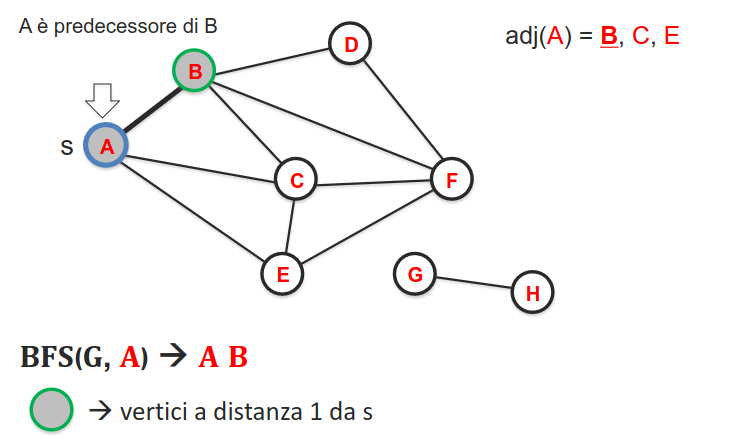
\includegraphics[width=80mm,scale=0.5]{bfs_esec2.png}
\end{center}
I vertici verdi indicano che la distanza dalla sorgente è 1.\\
Dopo aver visitato B, proseguo al secondo adiacente C, l'arco A-C diventa spesso 
perchè è stato percorso per scoprire C, inserisco C nella soluzione.\\
Passo ad E e faccio la stessa cosa.
\paragraph*{Coloro A di nero} Tutti gli adiacenti di A sono grigi (sono stati visitati), quindi
A diventa nero.
\paragraph*{Analizzo gli adiacenti di B}
\begin{center}
    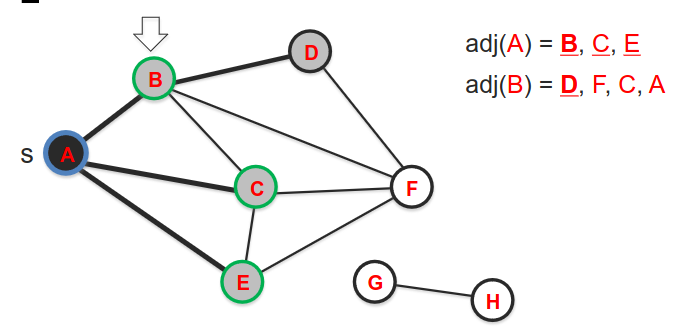
\includegraphics[width=80mm,scale=0.5]{bfs_esec3.png}
\end{center}
Osservo che gli adiacenti sono \ra $adj(B) = D,F,C,A$.\\
Analizzo D, noto che non è stato ancora esplorato (è bianco), quindi lo coloro di grigio e
faccio diventare l'arco B-D spesso. Coloro di Giallo il vertice D per indicare distanza 2 dalla
sorgente.\\
Lo stesso per F.\\
C lo ignoro perchè è stato già esplorato in precedenza.\\
A lo ignoro perchè è nero, quindi è già completo.\\
Notiamo che gli adiacenti di B sono tutti grigi, quindi B diventa nero.
\begin{center}
    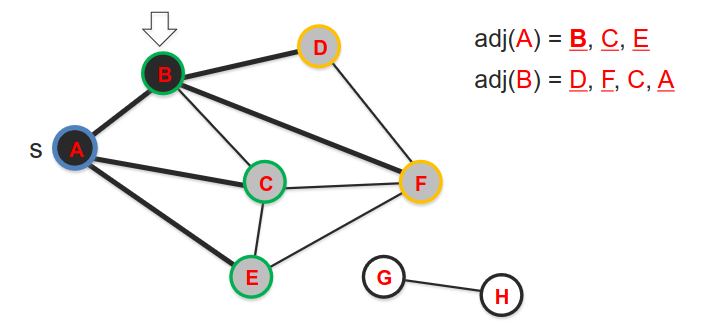
\includegraphics[width=80mm,scale=0.5]{bfs_esec4.png}
\end{center}
\paragraph*{Analizzo gli adiacenti a C} \ra $adj(C) = B,F,E,A$.\\
B lo ignoriamo perchè è nero.\\
F lo ignoriamo perchè è grigio.\\
E lo ignoriamo perchè è grigio.\\
A lo ignoriamo perchè è nero.
Tutti i vertici di C sono stati esplorati, C \ra nero.
\paragraph*{Analizzo gli adiacenti a E} \ra $adj(E) = A,C,F$.\\
A lo ignoro perchè è nero.\\
C lo ignoro perchè è nero.\\
F lo ignoro perchè è grigio.\\
Tutti i vertici di E sono stati esplorati, E \ra nero.
\paragraph*{Analizzo gli adiacenti di D} \ra $adj(D) = B, F$.\\
B lo ignoro perchè è nero.\\
F lo ignoro perchè è grigio.\\
Tutti i vertici di D sono stati esplorati, D \ra nero.
\paragraph*{Analizzo gli adiacenti a F} \ra $adj(F) = B,D,C,E$.\\
Tutti i vertici adiacenti sono neri.\\
Tutti i vertici di F sono stati esplorati, F \ra nero.
\begin{center}
    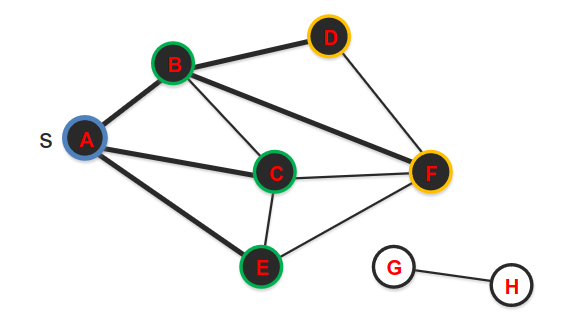
\includegraphics[width=80mm,scale=0.5]{bfs_esec5.png}
\end{center}
Questo è il risultato finale, notiamo che G e H, non sono stati esplorati, infatti sono bianchi.\\
Questo perchè BFS visita solo archi gli archi connessi alla sorgente.\\
A predecessore di B,C,E.\\
B predecessore di D,F.\\
Con questi dati otteniamo \textbf{l'Albero della BFS}:
\begin{center}
    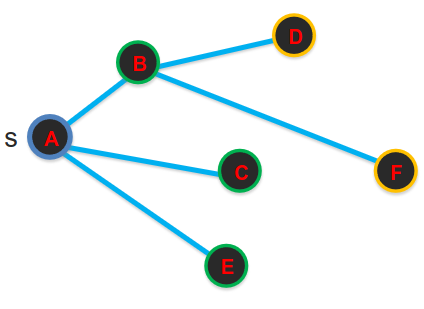
\includegraphics[width=80mm,scale=0.4]{bfs_albero.png}
\end{center}
\section{Strutture di base della BFS}
\begin{itemize}
    \item color \ra vettore dei colori
    \item d \ra vettore delle distanze
    \item $\pi$ \ra vettore dei predecessori
\end{itemize}
\subsection*{Vettore dei colori di lunghezza $|V|$}
color[v]:
\begin{itemize}
    \item W (bianco) \ra vertice non visitato
    \item G (grigio) \ra vertice visitato (ma non tutti gli adiacenti sono già
    stati ispezionati)
    \item B (nero) \ra vertice visitato (con tutti gli adiacenti visitati)
\end{itemize}
\paragraph*{Prima e Dopo la visita}
\begin{itemize}
    \item Prima della visita \ra color[v] = W per ogni vertice v
    \item Dopo la visita \ra color[v] = W per ogni vertice v non visitato
    \item Dopo la visita \ra color[v] = B per ogni vertice v visitato
\end{itemize}
\paragraph*{Durante la visita} un vertice v che ha ancora adiacenti da ispezionare è
di colore G. Nessun vertice ha colore G prima e dopo la visita.
\subsection*{Vettore delle distanze di lunghezza $|V|$}
d[v] \ra distanza di v dalla sorgente s.
\begin{itemize}
    \item Prima delle visita \ra $d[v] = \infty$ per ogni v diverso da s.
    \item Per la sorgente \ra $d[s] = 0$.
    \item Dopo la visita \ra $d[v] = \infty$ per ogni v non visitato.
    \item Dopo la visita \ra $d[v] = n$ per ogni v visitato distante n archi da s
\end{itemize}
\subsection*{Vettore dei predecessori di lunghezza $|V|$}
$\pi[v]=u$ \ra predecessore di v nella visita (si ha $(u,v)\in E$).
\begin{itemize}
    \item prima delle visita \ra $\pi[v] = NIL$ per ogni v
    \item dopo la visita \ra $\pi[s] = NIL$
    \item dopo la visita \ra $\pi[v] = NIL$ per ogni $v (\neq s)$ non visitato
\end{itemize}
\begin{box_giallochiaro}
    {color[v] = W dopo la visita $\implies d[v] = \infty$ e $\pi[v]=NIL$}.
\end{box_giallochiaro}
\subsection{BFS utilizza una coda Q}
\begin{itemize}
    \item Un vertice viene inserito in Q non appena viene visitato
    \item Un vertive visitato rimane in Q finchè non viene estratto per esplorare
    i suoi adiacenti
    \item Quando tutti gli adiacenti di un vertie risultano visistati, il vertice
    diventa nero
    \item la visita termina quando Q è vuota
\end{itemize}
Q contiene solo i vertici grigi!
\section{Operazioni sulla coda Q}
\begin{itemize}
    \item \textbf{head(Q)} restituisce il vertice in testa
    \item \textbf{enqueue(Q, v)}, inserisce il vertice v in coda
    \item \textbf{dequeue(Q)}, elimina il vertice in testa
\end{itemize}
\section{Codice}
\begin{lstlisting}[language=Java, escapeinside={!"}{"!}]
    Procedura_BFS(G, s)
        foreach v !"$\in$"! V \ {s} do
            color[v] = W, d[v] = !"$\infty,\, \pi[v]$"! = NIL
        color[s] = G, d[s] = 0, !"$\pi$"![s] = NIL
        Q = !"$\emptyset$"!
        enqueue(Q,s)
        while Q is not !"$\emptyset$"! do
            v = head(Q)
            foreach u !"$\in$"! adj(v) do
                if color[u] is W then
                    color[u] = G
                    enqueue(Q,u)
                    d[u] = d[v]+1
                    !"$\pi$"![u] = v
            color[v] = B
            dequeue(Q)
\end{lstlisting}
\subsection{Esempio esecuzione algoritmo BFS}
Nella slide 109 di BFS è riportata l'esecuzione passo per passo dell'algoritmo con
i valori di distanza e di colore per ogni vertice, riportando la variazione
passo per passo.\\
Risulta ancora più evidente che la coda contiene solo vertici grigi, dato che vengono inseriti
quando vengono scoperti e rimossi solo quando diventano neri.\\
La differenza con l'esecuzione grafica è che qua chiaramente al posto dei colori ci saranno le distanze
salvate nelle tabelle e il predecessore, quindi quando scopro un nuovo vertice
devo incrementare la distanza di 1 e aggiungere il vertice che sto analizzando 
(quello prelevato dalla coda tramite la head) come predecessore del vertice adiacente che
sto considerando (quello dentro il foreach).\\
Vediamo che grazie alla coda riusciamo a mantenere in memoria tutti i vertici grigi
e mano a mano che finiamo di analizzare i vertici effettuiamo la dequeue, quindi
quando la coda sarà vuota l'algoritmo termina.
\paragraph*{Alla fine dell'esecuzione avremo la seguente tabella}
\begin{center}
    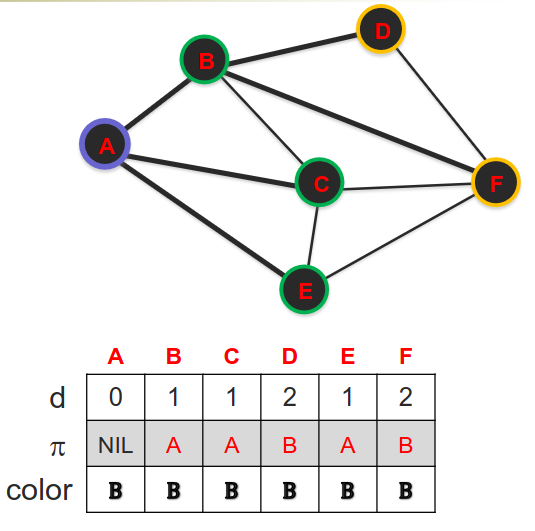
\includegraphics[width=80mm,scale=0.5]{bfs_tabella.png}
\end{center}
Per calcolare il il BFS Tree è sufficiente guardare quali sono i predecessori nella tabella,
questi sono i collegamenti che determinano l'albero di esplorazione BFS.
\subsection{BFS Tree}
$T = (V_T, E_T)$:
\begin{itemize}
    \item $V_T = \{v \in V | color[v] = B\}$
    \item $E_T = \{(\pi[v], v) | v \in V_T\}$
\end{itemize}
\subsection{Complessità in tempo}
$|V| \rt$ numero dei vertici del grafo.\\
$|E| \rt$ numero archi ndel grafo.--redirect-gateway def1
\begin{itemize}
    \item Costo di inizializzazione \ra $O(|V|)$
    \item Singola operazione su Q \ra tempo costante
    \item un vertice viene aggiunto a Q al più una volta
    \item un vertice viene estratto da Q al più una volta
    \item Ogni lista di adiacenza viene ispezionata quado il vertice viene estratto da Q
    (al più una volta)
    \item Dimebnsione totale delle liste di adiacenza \ra $2|E|$
    \item Costo di ispezioni delle liste di adiacenza \ra $O(|E|)$
\end{itemize}
\paragraph*{Complessità nel caso peggiore} $O(|V|+|E|)$
\section{Esercizi}
Sono stati proposti una serie di esercizi che richiedono l'utlizzo di BFS, per
esempio:
\paragraph*{Verificare se un grafo G=(V,E) è connesso}
\begin{lstlisting}[language=Java, escapeinside={!"}{"!}]
    Procedura Is_connected(G)
        u = randm vertex from V
        BFS(G,u)
        foreach v !"$\in$"! V do
            if colour[v] is W then
                return false
        return true
\end{lstlisting}

\chapter{Depth First Search (DFS)}
DFS(G), \textbf{Visità in profondità} di un grafo G:
\begin{itemize}
    \item Sceglie un vertice s come sorgente e visita s
    \item visita il prima adiacente $a_1$ di s, poi visita il primo adiacente $a_2$ di $a_1$,
    poi visita il primo adiacente $a_3$ di $a_2$, etc.
    \item Quando raggiunge un vertice che non ha adiacenti da visitare risale al predecessore
    e la visita riparte (se possibile) da n altro adiacente di tale predecessore
    \item Ogni volta che non ci sono adiacenti da visitare si risale al predecessore
    \item Quando la visita risale alla sorgente e s non ha più adiacenti da visitare, si sceglie
    una nuova sorgente e la visita riparte
    \item La visita termina quando non ci sono più vertici disponibili per essere scelti
    come nuova sorgente
\end{itemize}
\section{I colori dei vertici}
Anche in questo caso i vertici hanno associato un colore:
\begin{itemize}
    \item Vertice bianco \ra vertice non visitato
    \item Vertice grigio \ra vertice visitato (archi uscenti ancora da ispezionare)
    \item Vertice nero \ra vertice visitato (adiacenti completamente visitati)
\end{itemize}
Come per BFS.
\section{Utilizzo DFS}
Vedremo che DFS è ottimo nei grafi orientati, infatti vedremo esempi solamente di questo
tipo di grafo.
\paragraph*{Esempio DFS grafo orientato}
\begin{center}
    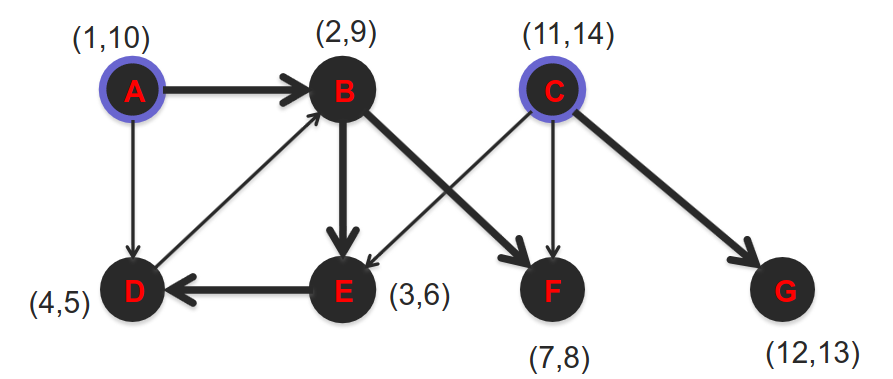
\includegraphics[width=80mm,scale=0.5]{dfs_esempio.png}
\end{center}
Notiamo che sui vertici sono presenti due valori:
\begin{itemize}
    \item Il primo è l'istante in cui il vertice viene scoperto, qua siamo partiti da A infatti viene
    riportato il valore 1
    \item Il secondo è l'istante in cui il vertice viene completato, quindi tutti i suoi
    adiacenti sono esplorati
\end{itemize}
\section{Struture di base}
DFS ha le seguenti strutture di base
\begin{itemize}
    \item color \ra vettore dei colori
    \item $\pi$ \ra vettore dei predecessori
    \item d \ra vettore dei tempi di scoperta
    \item f \ra vettore dei tempi di completamento
\end{itemize}
I colori sono gli stessi di BFS:
\begin{itemize}
    \item W bianco \ra vertice non visitato
    \item G grigrio \ra vertice visitato (non tutti gli archi uscenti sono stati ispezionati)
    \item B nero \ra vertice visitato (con tutti gli adiacenti visitati)
\end{itemize}
La differenza sta però nel colore dei vertici dopo la visita, perchè a differenza di BFS,
in questo caso dopo la visita non avrò nessun vertice W bianco, ma saranno tuti B neri.\\
Durante la visita chiaramente un vertice visitato, che han ancora archi uscenti da ispezionare
sarà grigio.
\subsection{Vettore dei predecessori}
$\pi[v]=u$ \ra predecessore di v nella visita $((u,v)\in E)$.
\begin{itemize}
    \item Prima della visita \ra $\pi[v] = NIL$ per ogni v.
    \item Dopo la visita \ra $\pi[v] = NIL$ per ogni v che è sorgente.
    \item Dopo la visita \ra $\pi[v] \neq NIL$ per ogni v che non è sorgente
\end{itemize}
\subsection{Vettore dei tempi}
\begin{itemize}
    \item \textbf{d[v]} \ra istante in cui v diventa grigio (scoperta)
    \item \textbf{f[v]} \ra istante in cui v diventa nero (completamento)
\end{itemize}
$d[v], f[v] \quad \in \quad \{1,2,...,2|V|\}$.\\
$d[v] < f[v]$ per ogni vertice v.\\
$[d[v], f[v]] \rt$ intervallo temporale di v.
\section{Teorema delle parentesi}
Graficamente se alla scoperta di un vertice associamo una parentesi aperta e
al completamente associamo una parentesi chiusa noteremo che alla fine le parentesi saranno
bilanciate.\\
Dopo una visita in profondità, uno solo dei tre casi seguenti si può verificare per
due vertici u e v:
\begin{enumerate}
    \item $[d[u],f[u]]$ contiene $[d[v],f[v]]$\\
    \ra v è discendente di u in un albero della visita
    \item $[d[v],f[v]]$ contiene $[d[u],f[u]]$\\
    \ra u è discendente di v in un albero della visita
    \item $[d[u],f[u]]$ e $[d[v],f[v]]$ sono disgiunti\\
    \ra u e v non sono discendenti l'uno dell'altro in un albero della visita
\end{enumerate}
\subsection{Proof del teorema}
\paragraph*{CASO 1 $d[u]<d[v]$} Cioè tempo di scoperta di u è minore del tempo di scoperta di v (viene
scoperto prima u di v)
\begin{enumerate}
    \item $d[v] < f[u]$ (cioè tempo di scoperta di v è minore del tempo di completamente di u)\\ 
    Verranno ispezionati tutti gli archi uscenti da v prima di riprendere l'ispezione
    degli archi uscenti da u.\\
    \ra v è discendente di u in un albero della visita, quindi \textbf{$f[v]<f[u]$}\\
    \ra $[d[u],f[u]]$ contiene $[d[v],f[v]]$
    \item $f[u]<d[v]$ (cioè u viene completato prima della scoperta di v)\\
    Sicuramente $d[u]<f[u]$ e $d[v] < f[v]$ \ra $d[u] < f[u] < d[v] < f[v]$\\
    Nessuno dei due vertici è stato scoperto mentre l'altro era grigio e quindi
    nessuno dei due vertci è discendente dall'altro nello stesso albero della visita.\\
    \ra $\boldsymbol{[d[u],f[u]]}$ e $\boldsymbol{[d[v],f[v]]}$ \textbf{sono disgiunti}
\end{enumerate}
\paragraph*{CASO 2 $d[u]>d[v]$} Si ripete scambiando i ruoli dei due vertici
\section{Etichettatura degli archi (grafo orientato)}
\paragraph*{Arco d'albero (arco T)} \ra Arco (u,v) tale che v è bianco quando
l'arco viene esplorato
\begin{center}
    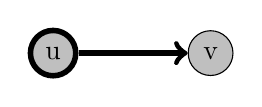
\begin{tikzpicture}
        \node[shape=circle,draw=black,line width=2pt,fill=lightgray] (A) at (0,0) {u};
        \node[shape=circle,draw=black,fill=lightgray] (B) at (2,0) {v};
    
        \path [line width=2pt, ->] (A) edge (B);
    \end{tikzpicture}
\end{center}
v viene visitato (e diventa grigio)\\
u diventa predecessore di v.
\paragraph*{Arco all'indietro (arco B)} \ra Arco (u,v) tale che v è grigio quando l'arco
viene esplorato.
\begin{center}
    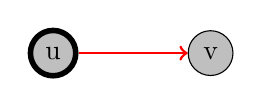
\begin{tikzpicture}
        \node[shape=circle,draw=black,line width=2pt,fill=lightgray] (A) at (0,0) {u};
        \node[shape=circle,draw=black,fill=lightgray] (B) at (2,0) {v};
    
        \path [line width=1pt, ->, draw=red] (A) edge (B);
    \end{tikzpicture}
\end{center}
u \underline{non} è predecessore di v nella visita\\
v è antenato di u nello stesso albero della visita \\ $\implies d[v] < d[u]$
\paragraph*{Arco in avanti (arco F)} \ra Arco (u,v) rale che, quando l'arco viene esplorato,
v è nero e $d[u] < d[v]$.
\begin{center}
    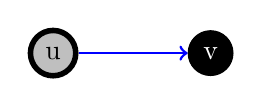
\begin{tikzpicture}
        \node[shape=circle,draw=black,line width=2pt,fill=lightgray] (A) at (0,0) {u};
        \node[shape=circle,draw=black,fill=black, text=white] (B) at (2,0) {v};
    
        \path [line width=1pt, ->, draw=blue] (A) edge (B);
    \end{tikzpicture}
\end{center}
u non è predecessore di v nella visita\\
u è antenato di v nello stesso albero della visita.
\paragraph*{Arco trasversale (arco C)} \ra arco (u,v) tale che, quando l'arco viene esplorato,
v è nero e $d[u] > d[v]$
\begin{center}
    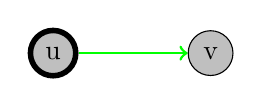
\begin{tikzpicture}
        \node[shape=circle,draw=black,line width=2pt,fill=lightgray] (A) at (0,0) {u};
        \node[shape=circle,draw=black,fill=lightgray] (B) at (2,0) {v};
    
        \path [line width=1pt, ->, draw=green] (A) edge (B);
    \end{tikzpicture}
\end{center}
u \underline{non} è predecessore di v nella visista.\\
u \underline{non} è antenato di v (e viceversa).\\
u e v possono anche fare parte di due diversi alberi della visita.
\subsection{Esempio di etichettatura archi}
\paragraph*{Esempio di Arco all'indietro}
\begin{center}
    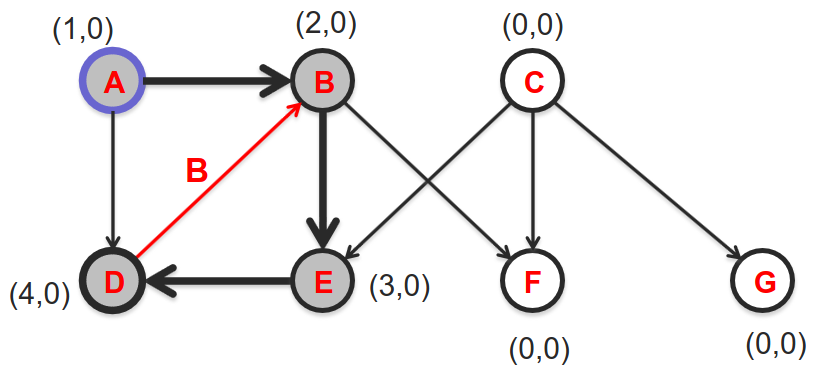
\includegraphics[width=80mm,scale=0.5]{dfs_arco_backward.png}
\end{center}
In questo caso analizzando il vertice D ci siamo trovati ad analizzare l'arco (D,B),
che parte da un arco grigio appena scoperto a uno grigio scoperto in precedenza (D non
è predecessore di B nella visista, B è antenato di B nello stesso albero della visista,
$d[D] < d[B]$). Si trata di un arco all'indietro.
\paragraph*{Esempio di arco in avanti}
\begin{center}
    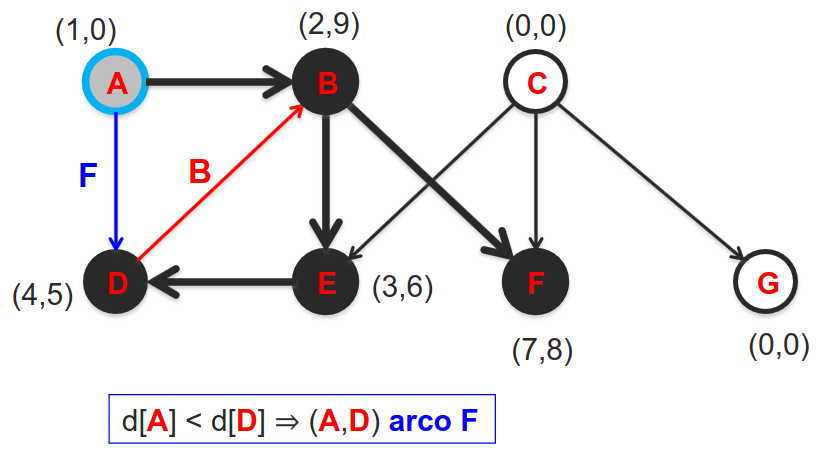
\includegraphics[width=80mm,scale=0.5]{dfs_arco_arco_in_avanti.png}
\end{center}
In questo caso notiamo che A è predecessore di D nella visista, infatti $d[A] < d[D]$ e
A è antenato di D, si tratto di un arco in avanti.\\
\paragraph*{Esempio di arco trasversale}
\begin{center}
    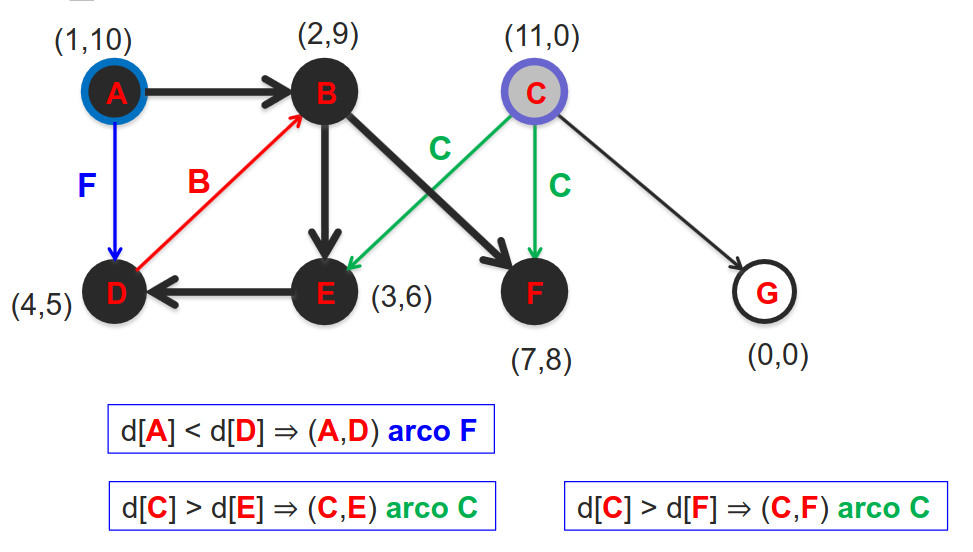
\includegraphics[width=80mm,scale=0.5]{dfs_arco_trasversale.png}
\end{center}
Notiamo in questo caso che i due archi (C,E) e (C,F), permettono di raggiungere vertici
appartenenti a un altro albero della visista, inoltre C non è predecessori di E, F nella
visista, C non è antenato di E,F (e vicevesrsa). Si tratta proprio di due archi trasversali.
\begin{center}
    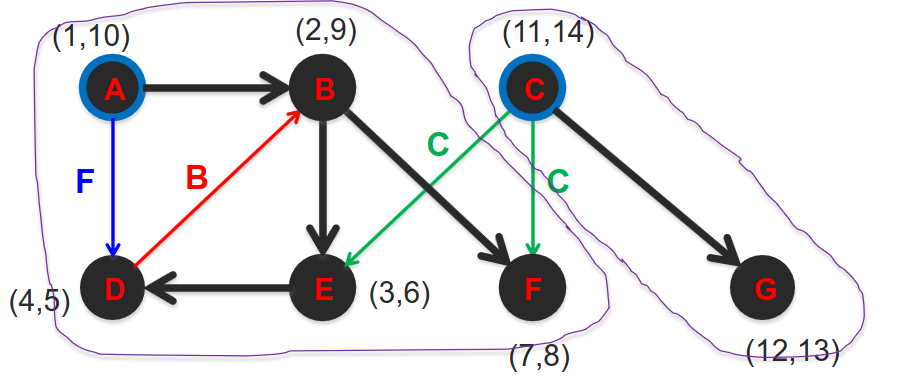
\includegraphics[width=80mm,scale=0.5]{dfs_dettaglio_archi_trasv.png}
\end{center}
In questa immagine notiamo ancor più nel dettaglio come gli archi trasversali tagliano i
2 alberi della visita.
\section{Algoritmo DFS}
\begin{lstlisting}[language=Java, escapeinside={!"}{"!}]
    Procedura DFS(G)
        // Inizializzazione vertici
        foreach v !"$\in$"! V do
            color[v] = W, !"$\pi[v]$"! = NUL, d[v] = 0, f[v] = 0
        time = 0
        foreach v !"$\in$"! V do
            if color[v] is W then
                DFS_visit(G,v)

    Procedura DFS_visit(G,u)
        time = time + 1
        d[u] = time, color[u] = G
        foreach v !"$\in$"! adj(u) do
            if color[v] = W then
                !"$\pi$"![v] = u
                DFS_visit(G,v)
        color[u] = B
        time = time + 1
        f[u] = time
\end{lstlisting}
Notiamo che l'approccio DPS si presta ad essere risolto tramite ricorsione, infatti 
il ragionamento è se il vertice adiacente è W allora visita tramite DFS quel vertice e così via,
fino a quando arrivo a un vertice senza adiacenti, allora torno indietro fino a quando
trovo un adiacente non esplorato.
\paragraph*{Complessità in tempo} $|V|$ \ra numero dei vertici del grafo\\
$|E|$ \ra numero degli archi del grafo:
\begin{itemize}
    \item Costo di inizializzazione \ra $O(|V|)$
    \item DFS\_visit(G,v) viene chiamata al più una volta per ogni vertice v del grafo \ra
    $O(|V|)$ chiamate
    \item Complessivamente su tutte le chimate di DFS\_visit(G,v), il costo di ispezione 
    delle liste di adiacenza è $O(|E|)$
\end{itemize}
\textbf{Complessità nel caso peggiore} $O(|V|+|E|)$.
\subsection{Modifica codice per aggiungere etichettatura archi}
Chiaramente la parte da modificare sarà quella relativa all'analisi degli adiacenti
quindi:
\begin{lstlisting}[language=Java, escapeinside={!"}{"!}]
    Procedura DFS_visit(G,u)
        time = time + 1
        d[u] = time, color[u] = G
        foreach v !"$\in$"! adj(u) do
            if color[v] = W then
                (u,v) = "Arco T"
                !"$\pi$"![v] = u
                DFS_visit(G,v)
            else 
                if color[v] = G then
                    (u,v) = "Arco B"
                else
                    if d[u] < d[v] then
                        (u,v) = "Arco F"
                    else
                        (u,v) = "Arco C" 
        color[u] = B
        time = time + 1
        f[u] = time
\end{lstlisting}
\section{Ordinamento Topologico}
Si consideri un grafo G=(V,E) orientato aciclico (Directed Acyclic Graph, DAG).\\
L'ordinamento topologico è un elenco dei vertici:
\[ T = \langle v_1,v_2,v_3,...,v_n \rangle \]
tale che per ogni arco ($v_i, v_j$) si ha che $v_i$ viene prima di $v_j$ in T.\\
In poche parole dobbiamo stampare i vertici nell'ordine con cui sono stati completati.
\begin{center}
    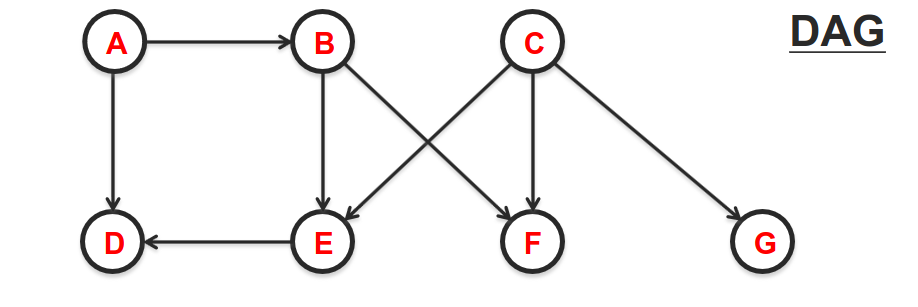
\includegraphics[width=80mm,scale=0.5]{dfs_ord_topologico.png}
\end{center}
In questo esempio (grafo simile al precedente, è stato eliminato un arco per rendere il grafo
aciclico), abbiamo che l'ordinamento è 
\[ T = \langle C, G,A,B,F,E,D \rangle \]
che sarebbe l'ordine dall'ultimo vertice completato al primo.
\begin{center}
    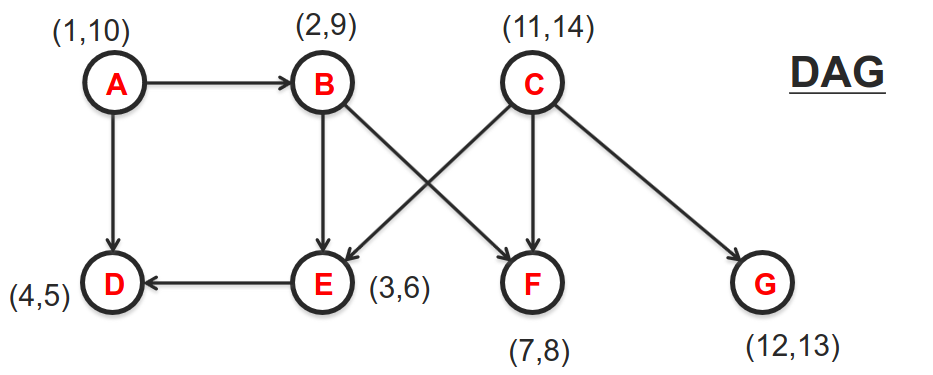
\includegraphics[width=80mm,scale=0.5]{dfs_ord_topologico_2.png}
\end{center}
Guardando il grafo con i tempi di scoperta e di completamento notiamo infatti che C
ha tempo di completamento massimo (14), ripercorrendo a ritroso ritroviamo G (13), poi
A (10), e così via.\\
Per calcolare questa lista la struttura dati ideale è una pila, dato che quando completiamo un vertice
ci basterà inserirlo nella pila effetuando una push, così a fine esecuzione troveremo in cima alla pila l'ultimo
vertice completato, ci basterà effettuare la pop di ogni elemento stampandolo e otterremo così
la lista dell'ordinamento topologico.\\
\subsection{Codice}
Ci basterà aggiungere le funzioni per inizializzare la pila e ogni volta che un vertice
verrà completato effettuare la push dello stesso sulla pila e infine stampare tutti gli elementi
effettuando le pop fino a quando la lista non è vuota.
\begin{lstlisting}[language=Java, escapeinside={!"}{"!}]
    Procedura DFS(G)
        // Inizializzazione vertici
        foreach v !"$\in$"! V do
            color[v] = W, !"$\pi[v]$"! = NUL, d[v] = 0, f[v] = 0
        time = 0
        S = empty stack // Inizializzazione pila
        foreach v !"$\in$"! V do
            if color[v] is W then
                DFS_visit(G,v)
        // Stampa ordinamento
        while not isEmpty(S) do 
            print top(S)
            pop(S)

    Procedura DFS_visit(G,u)
        time = time + 1
        d[u] = time, color[u] = G
        foreach v !"$\in$"! adj(u) do
            if color[v] = W then
                !"$\pi$"![v] = u
                DFS_visit(G,v)
        color[u] = B
        push(S,u) //push del vertice completato
        time = time + 1
        f[u] = time
\end{lstlisting}
\section{Visita in profondità di un grafo non orientato}
Nelle slide notiamo come l'ordine di visita rispetto allo stesso grafo, ma orientato
cambia, perchè chiaramente prima per raggiungere alcuni vertici dovevo attendere la selezione
di una nuova sorgente, in questo caso invece esploro tutto partendo da A.\\
Notiamo anche che sono presenti solo archi T (d'albero) e archi B (all'indietro), perchè
in un grafo non orientato non posso avere archi in avanti e archi trasversali, dato che sono
concetti che hanno senso in presenza di un grafo orientato.
\subsection{Codice}
Essendo un grafo non orientato devo stare attento a non visistare il predecessore, dato che
esso compare nella lista dei predecessori, quindi non va considerato e va escluso dalla lista
degli adiacenti, soprattutto in vista dell'etichettatura degli archi.
\begin{lstlisting}[language=Java, escapeinside={!"}{"!}]
    Procedura DFS(G)
        // Inizializzazione vertici
        foreach v !"$\in$"! V do
            color[v] = W, !"$\pi[v]$"! = NUL, d[v] = 0, f[v] = 0
        time = 0
        foreach v !"$\in$"! V do
            if color[v] is W then
                DFS_visit(G,v)

    Procedura DFS_visit(G,u)
        time = time + 1
        d[u] = time, color[u] = G
        // Togliamo il predecessore dagli adj
        foreach v !"$\in$"! adj(u) \ {!"$\pi[u]$"!} do
            if color[v] = W then
                !"$\pi$"![v] = u
                (u,v) = "Arco T"
                DFS_visit(G,v)
            else
                (u,v) = "Arco B" 
        color[u] = B
        time = time + 1
        f[u] = time
\end{lstlisting}
